\subsection{Introducción}\label{header-n2}

OpenFOAM \emph{(Open Field Operation And Manipulation)} es un código
para la resolución de problemas CFD en continuo desarrollo, de fuentes
abiertas, robusto y avanzado, ampliamente usado en la industria. El
paquete incluye módulos para una amplia gama de aplicaciones. Algunas de
sus características más relevantes son:

\begin{itemize}
\item
  Las fuentes son libres y abiertas, con lo que está disponible sin
  costes de licencia y se puede modificar y adaptar el código.
\item
  Las librerías están escritas en lenguaje C++, orientado a objetos, con
  estructura modular que facilita programar nuevos resolvedores,
  condiciones de entorno y la compatibilidad con diversas aplicaciones,
  no siendo necesaria una profundización extensa en la amplitud del
  código.
\item
  Preparado para correr los casos en paralelo, mediante métodos de
  cálculo fáciles de establecer y de calcular, manejando por sí la
  descomposición del proceso y la reconstrucción final.
\item
  Está diseñado para resolver problemas complejos, soportando fluidos en
  dos fases con variedad de modelos de turbulencia (Ej. Modelo RAS
  (Reynolds-Averaged Stress), LES (Large-Eddy Simulation), k-w SST(Shear
  Stress Transport)).
\item
  Al igual que la mayoría de los programas para el análisis
  computacional de la Mecánica de Fluidos, usa una discretización de
  volúmenes finitos. Este método describe cada fase con la fracción alfa
  (alfa=1 todo agua, alfa=0 aire) por el volumen ocupado del fluido en
  cada celda.
\item
  Para el preproceso y postproceso se pueden utilizar aplicaciones
  auxiliares para las cuales existen órdenes directas de conversión
  listadas en la Guía de Usuario.
\item
  Además, se añade el paquete de terceros (\emph{Thitd Party}), el cual
  implementa el programa ParaView, software principal usado para el
  postproceso.
\end{itemize}

\subsection{Trayectoria de OpenFOAM}\label{header-n28}

FOAM fue escrito por Henry Weller, entre otros, en el Imperial Collage
en 1989. Entre los años 2000-2004 FOAM fue un código comercializado por
la compañía Nabla Ltd. No obstante, en 2004 decidieron lanzar el código
bajo licencia GPL con el nuevo nombre de OpenFOAM. Este se distribuyó
por OpenCFD durante varios años, pero en 2011 SGI compró OpenCFD. Poco
después, en 2012, SGI vendió OpenCFD y la marca OpenFOAM a ESI Group.

Algunos miembros del grupo que desarrollaron FOAM, decidieron crear
\href{http://www.openfoam.org/contrib/}{"The OpenFOAM Fundation"} para
continuar desarrollando el código, corregir errores, ofrecer cursos y
consultorías especializadas. Desde entonces, lanzan una nueva versión
cada 6 meses, \href{https://openfoam.org/download/history/}{Release
History}. Como se ha mencionado, la marca OpenFOAM pertenece a OpenCFD
Ltd, pero se la concedieron a la fundación para su uso. Las versiones
publicadas, son de alta calidad, comprobadas (\emph{future-proof}) y
fáciles de mantener. No obstante, su política de aceptación de
contribuciones es bastante estricta, lo que reduce las aportaciones por
la comunidad en desarrollos que pudieran estar disponibles e
implementados en la distribución. Esto recientemente ha cambiado, más
adelante se detalla la estrategia para ofrecer más soporte.

En cambio
\href{https://www.cfd-online.com/Forums/openfoam-news-announcements-opencfd/165324-opencfd-pleased-announce-release-openfoam-v3-0-a.html}{OpenCFD
Ltd} tiene su propio ciclo de desarrollo, proporcionando nuevas
características, tratando de mantener los mismos estándares.

En 2016, utilizando como base la versión de \emph{OpenFOAM Fundation},
se añadieron nuevas funcionalidades, fruto del desarrollo por clientes
de OpenCFD y por la comunidad de OpenFOAM. Esto dió lugar a otra línea
de desarrollo del código
\href{http://www.openfoam.com:80/version-v1606+/}{OpenFOAM 1606+}
(\href{https://web.archive.org/web/20170622010404/http://www.openfoam.com:80/version-v1606+/}{The
way back machine}) (YearMonth+, ISO-8601).

El primer indicio de OpenFOAM+ se hizo público, en octubre de 2015, con
la versión de OpenFOAM para Windows, y más tarde basado en la línea de
desarrollo 3.0, cohexistieron OpenFOAM 3.0 y OpenFOAM 3.0+, lo que
confundió a la comunidad
\href{https://www.cfd-online.com/Forums/openfoam/165322-openfoam-v3-0-a.html}{OpenFOAM
v3.0+ ??} y conllevó a la nueva nomenclatura, mencionada anteriormente.
A parte de las explicaciones que se dieron por la comunidad, en el
siguiente blog se aclaran las diferentes ramas desarrolladas entorno al
programa,
\href{https://sites.google.com/view/olaflowcfd/blog/old-blog-entries/what-is-what-and-who-is-who-in-the-openfoam-environment}{\emph{What
is what and who is who in the OpenFOAM environment?}}.

\begin{figure}
\centering
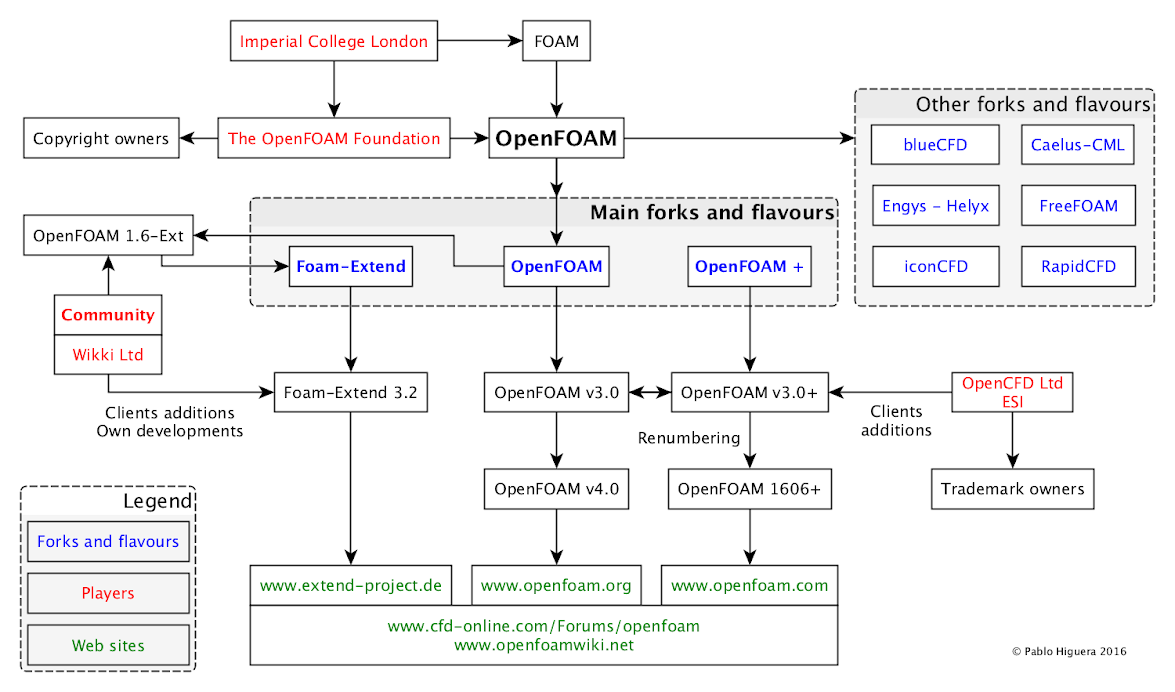
\includegraphics{41-historyOF.png}
\caption[Esquema de la trayectoria del desarrollo del código]{Esquema de la trayectoria del desarrollo del código \cite{higuera16}}
\label{fig:historyOF}
\end{figure}

OpenCFD Ltd (ESI Group) sigue distribuyendo el código gratuitamente bajo
licencia GPL. Además, como puede verse entre las novedades, hace no
mucho publicaron una nueva versión\footnote{
\href{https://www.openfoam.com/news/}{Main OpenFOAM News}}, concretamente
\href{https://www.openfoam.com/releases/openfoam-v1706/}{31/12/2017
OpenFOAM v1706}, la cual cuenta con numerosas contribuciones de:

\begin{itemize}
\item
  \href{http://www.wikki.co.uk/}{Wikki}
\item
  \href{https://cfmesh.com/company/}{Creative Fields}
\item
  \href{http://openfoam.org}{OpenFOAM Fundation}\\
\item
  Instituto de Hidráulica Ambiental
  \href{http://www.ihcantabria.com/en/}{IHCantabria}
\item
  \href{http://www.cfd-berlin.com/}{CFD Software E+F GmbH}
\end{itemize}

Para que el software de código abierto evolucione y prospere, se
necesita de la comunidad. La financiación también es necesaria, por ello
desde la Fundación de OpenFOAM se reunen diferentes objetivos dentro del
llamado \href{https://openfoam.org/news/funding-2018/}{Mantenimiento de
OpenFOAM}.

En 2016 se llevó a cabo una campaña que concluyó de forma exitosa para
recaudar \euro{}100k de fondos para el 2017. Esto sirvió para financiar,
mejoras en el código, resolución de informes de errores, paquetes
compatibles con sistemas operativos Linux y macOS y el lanzamiento de
OpenFOAM v5.

Las actividades mencionadas, forman parte de los costes recurrentes para
mantener OpenFOAM entre los estándares más altos y evolucionar en la
dirección de las expectativas de los usuarios. Los costes anuales son de
aproximadamente \euro{}250k incluyendo lo siguiente:

\begin{itemize}
\item
  \euro{}80k- Desarrollos entorno a la usabilidad: nuevos códigos,
  ejemplos de casos y documentación.
\item
  \euro{}60k- Rediseño del código: modificando la estructura para
  integrar nuevos desarrollos.
\item
  \euro{}60k- Resolución de errores: anualmente gestionan 500 informes
  de problemas, resolviendo funcionalidades incorrectas/incompletas.
\item
  \euro{}25k- Distribución y comprobaciones: creando casos, ejecutando
  comprobaciones, compilación del código, lanzamiento de nuevas
  versiones y promoción.
\item
  \euro{}25k- Fase de operación: \emph{marketing} , infraestructura de
  la web, cumplimiento y aplicación de licencias, finanzas y
  administración, consultas generales.
\end{itemize}

\begin{figure}
\centering
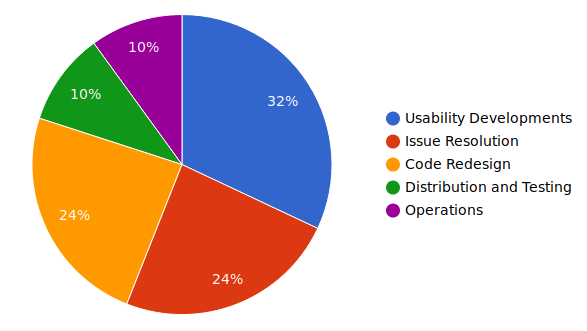
\includegraphics{42-FondosOF.png}
\caption[Distribución de costes]{Distribución de costes - The OpenFOAM Fundation \href{https://openfoam.org/news/funding-2018/}{Fuente}}
\end{figure}

Para lograr los fondos necesarios para el mantenimiento, en 2018
introdujeron los \href{https://openfoam.org/maintenance/}{Planes de
Fondos OpenFOAM}. Así, lograron compromisos por parte de
\href{https://openfoam.org/supporters/}{organizaciones de apoyo} con la
adquisición de estos planes, además, las organizaciones comercialmente
dependientes del código (las cuales obtienen ahorros significativos en
tarifas de licencias) pueden apoyar su desarrollo y priorizar las
solicitudes enviadas.

\subsection{Instalación de OpenFOAM}\label{header-n91}

Las instrucciones a seguir para la instalación dependerán del sistema
operativo que se vaya a utilizar, principalmente está pensado para
distribuciones de Linux, aunque también se incluyen instrucciones para
arrancar el programa desde Windows o Mac soportado desde Docker.

A lo largo de los años se han realizado muchas mejoras, se han añadido
funcionalidades, se ha reescrito parte del código, etc., por ello es
recomendable trabajar con la última versión estable del programa.
Además, cabe destacar que progresivamente se ha mejorado el tiempo que
conlleva el proceso de instalación.

Durante el transcurso de las simulaciones se ha trabajado con diferentes
versiones. No obstante, los cambios necesarios para adecuar un caso de
una versión a otra pueden detectarse fácilmente comparando el mismo caso
de tutorial mediante alguna herramienta de comparación de archivos (como
\emph{WinMerge} o \emph{meld}).

Adicionalmente, si se opta por usar
\href{https://docs.docker.com/docker-for-windows/}{Docker}, este permite
ejecutar desde terminal o desde
\href{https://github.com/portainer/portainer}{portainer} un entorno
personalizado (comúnmente conocido como un \emph{contenerdor}) que
incluye la \emph{imagen} del código, además de herramientas y librerias
necesarias para procesar y visualizar el caso. Así mismo, esta
herramienta utiliza toda la potencia del ordenador (a partir de la
versión de windows 10).

\subsection{Estructura de un caso}\label{header-n103}

Un caso es un conjunto de carpetas y archivos que definen un problema
específico de ingenieria y la forma en que se va a resolver. La
esturctura mínima de ficheros necesaria para poder solucionar un
fenómeno es: \texttt{constant}, \texttt{system} y \texttt{0} (una
carpeta temporal inicial). Esta última no tiene porque corresponder con
el tiempo \emph{0} ya que el caso puede ser una parte de un proceso que
haya sido simulado previamente.

Dependiendo del tipo de solver y del tipo de problema a tratar se
necesitará una mayor o menor cantidad de archivos auxiliares.

En \textbf{system} se incluyen archivos relacionados con el proceso de
resolución: \emph{blockMeshDict} (contiene información sobre el modelo y
los contornos), \emph{controlDict} (es donde se establecen los
parámetros relacionados con el tiempo de resolución, paso del tiempo, o
funciones para resolver los campos de variables específicaspor cada
iteración), \emph{fvSchemes}(describe los esquemas numéricosutilizados
para resolver el sistema de ecuaciones), y \emph{fvSolution} (determina
cómo se solucionarán las ecuaciones contenidas en fvSchemes, qué método
de acoplamiento/algoritmo se emplea, así como, el esquema para la
solución de las variables a calcular y las tolerancias).

En el directorio \textbf{constant} se encuentran los ficheros donde se
describen las propiedades físicas de los flujos (diccionario
\emph{transportProperties}), fuerzas exteriores (\emph{g}) y los modelos
de turbulencia (\emph{turbulenceProperties}).

\subsection{Pasos para resolver un problema CFD}\label{header-n114}

Como ya se ha mencionado, la simulación CFD permite obtener más
precisión en los resultados, ofreciendo buenas estimaciones de lo que
sucederá en la realidad. Para ello, es muy importante definir
adecuadamente los parámetros del caso, así como la \emph{escala de
flujo} requerida. Esta escala, está condicionada por la longitud del
dominio, la velocidad y el tiempo de simulación. Es decir, se debe
retener en el modelo sólo las partes relevantes; si se define bien el
dominio la solución convergerá adecuadamente.

El parámetro adimensional que relaciona estas variables, es el número de
Reynolds, si se quisiera aumentar este número, sería necesario bajar la
temperatura o aumentar la presión del dominio. A medida que se aumente
el número de Re o la escala de flujo, se requerirán más recursos
computacionales.

El \textbf{teorema de \(\pi\) de
\href{https://es.wikipedia.org/wiki/Teorema_\%CF\%80_de_Vaschy-Buckingham}{Vaschy-Buckingham}}
es el teorema fundamental del análisis dimensional. El teorema establece
que dada una relación física expresable mediante una ecuación en la que
están involucradas \emph{n} magnitudes físicas o variables, y si dichas
variables se expresan en términos de \emph{k} cantidades físicas
dimensionalmente independientes, entonces la ecuación original puede
escribirse equivalentemente como una ecuación con una serie de
\emph{n-k} números adimensionales construidos con las variables
originales. Este teorema explica que si se quisiera realizar una
simulación a escala, sin cambiar la temperatura ni la gravedad, las
dimensiones también deberían ser iguales, luego físicamente no tendría
sentido.

\subsubsection{Preproceso}\label{header-n123}

\paragraph{Geometría del caso}\label{header-n126}

En OpenFOAM el mallado se carga a través de la orden
\href{http://cfd.direct/openfoam/user-guide/blockMesh/\#x25-1420005.3}{blockMesh}
o
\href{http://cfd.direct/openfoam/user-guide/snappyHexMesh/\#x26-1520005.4}{snappyHexMesh}.
La primera opción, resulta sencilla de interpretar y de manipular cuando
se trata de geometrías sencillas; pero cuando los diseños se vuelven
algo más complejos se suele utilizar la segunda opción. Esta última
opción implica la adición de un fichero, ubicado en
\textless{}./constant/triSurface/\textgreater{}, el cual contenga la
geometría del modelo en STL (STereo Lithography).

Las órdenes, ejecutadas por terminal, leen el diccionario
correspondiente, ubicado en
\textless{}./system/blockMeshDict\textgreater{} o
\textless{}./system/snappyHexMeshDict\textgreater{}, el cual determina
la geometría del dominio computacional a estudiar, mediante la
definición de los vértices, caras, celdas, bloques y contornos del caso.
Su funcion principal es la descomposición del dominio en sus tres ejes
por hexaedros.

OpenFOAM siempre opera en 3D, para ejecutar un caso en 2D se debe
especificar la condición \texttt{empty} en las áreas normales a la
dirección del eje para el cual no se requerirá una solución.

Adicionalmente, existen otras muchas opciones para realizar el mallado a
través de diferentes programas que luego OpenFOAM podrá reconocer. La
lista de los softwares, que cuentan con una orden directa para ser
exportados, se encuentran en la
\href{http://www.openfoam.org/features/mesh-conversion.php}{tabla de
conversión} de malla.

\paragraph{Propiedades físicas}\label{header-n137}

La información acerca de la viscosidad cinemática (\emph{nu}) y densidad
(\emph{rho}) de los fluidos presentes en el caso se determinan en el
fichero \textless{}./constant/transportProperties\textgreater{}. Las
dimensiones de las variables se expresan de la forma explicada en
\href{https://cfd.direct/openfoam/user-guide/basic-file-format/\#x17-1290004.2.6}{User
Guide: 4.2.6 Dimensional units}.

Por otro lado, las fuerzas exteriores que intervienen en este problema,
en este caso la gravedad, se define en
\textless{}./constant/g\textgreater{}, con una dirección negativa en la
componente \emph{y}.

\paragraph{Modelado de la turbulencia}\label{header-n144}

El modelo de turbulencia para el caso se implementa en el diccionario
\textless{}./constant/turbulenceProperties\textgreater{}, pueden ser:

\begin{enumerate}
\def\labelenumi{\arabic{enumi}.}
\item
  laminar: no usa modelo de turbulencia;
\item
  RAS: Reynolds-averaged simulation;
\item
  LES: Large eddy simulation.
\end{enumerate}

En este estudio se simulará el caso con los dos primeros, dado que son
los más comunes en este tipo de problemas. Como el modelo consta de una
pared contra la que el agua colisionará, el modelo RAS ofrecerá una
mayor aproximación a la realidad. Para este modelo se requerirán las
siguientes entradas:

\begin{itemize}
\item
  \texttt{RASModel}: nombre del modelo de turbulencia RAS. En los casos
  que se simularán se implementa \texttt{kEpsilon}, modelo estandar de
  turbulencia para flujos incompresibles y compresibles, incluyendo la
  teoría de distorsión rápida (rapid distortion theory, RDT) por el que
  se basa el término de compresión (\emph{based compression term}).
\item
  \texttt{turbulence}: activar la resolución del modelamiento de la
  turbulencia.
\item
  \texttt{printCoeffs}: devolver por terminal los coeficientes del
  modelo al comienzo de la simulación.
\item
  \texttt{\textless{}RASModel\textgreater{}Coeffs}: diccionario opcional
  de coeficientes para el respectivo modelo RAS.
\end{itemize}

\paragraph{Condiciones inciales y de
contorno}\label{header-n175}

Las condiciones se establecen en la carpeta
\textless{}./0\textgreater{}, la cual contiene las condiciones de
contorno e iniciales de todas las variables primarias que intervienen en
el problema físico, así como sus respectivas magnitudes.

La definición de los contornos es un tema bastante complejo porque su
papel en el modelado no consiste simplemente en el modelado de una
entidad geométrica, sino en una parte integral de la solución a través
de las condiciones de contorno o "conexiones" inter-fronterizas.

Para ver la lista completa de los tipos disponibles en OpenFoam:

\begin{itemize}
\item
  Para ``alpha.water'' se especifica el tipo \texttt{zeroGradient} en
  todas las áreas, para expresar un valor nulo en el gradiente de la
  componente normal a la pared, salvo para la parte superior
  (atmosphere) para la cual se determina la condición
  \texttt{inletOutlet}, que se trata de una derivación de
  \texttt{mixes}, la cual cambia entre \texttt{zeroGradient} cuando el
  fluido fluye fuera del dominio por una cara, y \texttt{fixedValue},
  cuando el fluido entra en el dominio.
\item
  Para la ``p'' se utiliza el tipo \texttt{fixedFluxPressure}, esta
  condición de contorno se usa cuando hay zonas \texttt{zeroGradient}, y
  donde las fuerzas del cuerpo, como la gravedad y la tensión
  superficial están presentes en las ecuaciones de la solución. Para la
  atmósfera, se usa una combinación de la condición
  \texttt{totalPressure} para la presión y
  \texttt{pressureInletOutletVelocity} para la velocidad, donde la
  velocidad del flujo de entrada es desconocida, pero la presión es
  conocida.
\item
  Para la ``U'' se selecciona una condición \texttt{noSlip} para todas
  las paredes, donde la componente normal será cero.
\item
  Los parámetros de la turbulencia, como "k" o "epsilon", también se
  definen en esta carpeta. Las paredes, típicamente, se definen como
  \texttt{WallFunction}, y para la atmosfera se utiliza el tipo
  \texttt{inletOutlet}. Para verificar las propiedades de turbulencia,
  se puede utilizar la calculadora de
  \href{http://www.cfd-online.com/Tools/turbulence.php}{turbulencia CFD}
  en línea.
\end{itemize}

En este caso se agrega el diccionario
\textless{}./system/setFieldsDict\textgreater{}, con el cual se
introcuce el volumen ocupado por el agua en el instante inicial. Hay
diferentes formas de determinar este volumen, para el caso a estudio se
usa \texttt{boxToCell} un bloque definido por una diagonal. Se
recomienda que las dimensiones sobrepasen el dominio en las zonas donde
el agua ocupe el volumen hasta la pared, ya que OpenFoam solo calculará
la fracción de fase dentro del dominio computacional.

\paragraph{Esquemas de discretización}\label{header-n199}

Ubicado en el directorio \textless{}./system/\textgreater{}, en el
fichero
\href{http://cfd.direct/openfoam/user-guide/fvschemes/}{fvSchemes} se
configuran los esquemas de discretización, en particular el esquema de
integración temporal y los esquemas de convección (transporte).

Esquema para la integración de tiempo:

\begin{itemize}
\item
  \texttt{steadyState}: establece las derivadas del tiempo a cero.
\item
  \texttt{Euler}: transitorio, implicito de primer orden, estable.
\item
  \texttt{backward}: transitorio, implicito de segundo orden,
  potencialmente inestable.
\item
  \texttt{CrankNicholson}: transitorio, implicito de segundo orden,
  estable.
\end{itemize}

Esquemas de interpolación, gradiente, divergencia y Laplacianos:

\begin{itemize}
\item
  \texttt{linear}: Diferencia central de segundo orden (\emph{second
  order central difference}).
\item
  \texttt{cubic}: Diferencia central de cuarto orden (\emph{Fourth order
  central difference}).
\item
  \texttt{upwind}: "\emph{upwind}" de primer orden (\emph{First order
  upwind}).
\item
  \texttt{linearUpwind}: "\emph{upwind}" de primer/segundo orden
  (\emph{First/second order upwind}).
\end{itemize}

\paragraph{Procedimiento de resolución}\label{header-n233}

En el fichero
\href{http://cfd.direct/openfoam/user-guide/fvSolution/\#x20-1450004.5.1}{fvSolution},
ubicado en \textless{}./system/\textgreater{}, se definen y configuran
los resolvedores lineales matriciales para la fracción de fase
\emph{alpha}, el campo de velocidades \emph{U} y de presiones \emph{p}:

\begin{itemize}
\item
  \texttt{PCG/PBiCG}: Preconditioned (bi-)conjugate gradient, PCG para
  mallas simétricas, PBiCG para mallas asimétricas.
\item
  \texttt{smoothSolver}: Emplea un refinado (ej. Gauss-Seidel).
\item
  \texttt{GAMG}: Generalised geometric-algebraic multi-grid.
\end{itemize}

Además de los resolvedores lineales, en este fichero se especifica el
algoritmo o método de acoplamiento a emplear para hallar los valores
para cada campo (SIMPLE, PISO o PIMPLE).

\subsubsection{Proceso}\label{header-n250}

\paragraph{Control del tiempo}\label{header-n253}

Los parámetros, como el tiempo que tarda en leer y escribir una
solución, se determinan en
\textless{}./system/controlDict\textgreater{}. El parámetro adimensional
del número de Courant relaciona, el paso del tiempo, la velocidad del
flujo por una celda y el tamaño de la celda. Tal y como se describe en
\href{https://cfd.direct/openfoam/user-guide/controlDict\#x18-1370004.3}{User
Guide 4.3: Time and data input/output control}, estas variables se
definen en el código de la siguiente manera:

\begin{itemize}
\item
  \textbf{startFrom}: Controla el tiempo de comienzo de la simulación.

  \begin{itemize}
  \item
    \texttt{firstTime}: Paso del tiempo más temprano del conjunto de
    directorios de tiempo.
  \item
    \texttt{startTime}: El tiempo se especifica por la entrada
    \emph{startTime}
  \item
    \texttt{latestTime}: Paso del tiempo más reciente desde el
    conjununto de directorios de tiempo.
  \end{itemize}
\item
  \textbf{startTime}: Comienzo de la simulación con
  \texttt{startFrom\ startTime}.
\item
  \textbf{stopAt}: Controla el tiempo de finalización de la solución.

  \begin{itemize}
  \item
    \texttt{endTime}: El tiempo se especifica con la entrada
    \emph{endTime}
  \item
    \texttt{writeNow}: Detiene la simulación al completar el paso del
    tiempo actual y escribe los datos.
  \item
    \texttt{noWriteNow}: Detiene la simulación al completar el paso del
    tiempo actual pero no escribe los datos.
  \item
    \texttt{nextWrite}: Detiene la simulación al completar el próximo
    tiempo de escritura programado, especificado por el diccionario
    \emph{writeControl}.
  \end{itemize}
\item
  \textbf{endTime}: El final de la simulación se da cuando
  \texttt{stopAt\ endTime}.
\item
  \textbf{deltaT}: Paso del tiempo de la simulación.
\end{itemize}

\paragraph{Escritura de datos}\label{header-n297}

En el fichero de \textless{}./system/controlDict\textgreater{}
mencionado en el apartado anterior, también viene definido el control
sobre cada cuanto se guarda la solución:

\begin{itemize}
\item
  \textbf{writeInterval}: este parámetro corresponde al número de
  ficheros de tiempo que se obtendrán por cada paso de tiempo a lo largo
  de la simulación. Es decir, si se quieren los resultados cada
  \((0,1-0,2-...-0,5)s\) con un paso del tiempo de \(\delta t=0,005s\),
  se necesita una salida de resultados de \(writeInterval=20\)
  (tiempos).
\item
  \textbf{writeControl}: cuando se requiere alguna modificación de los
  parámetros, durante la ejecución de una simulación, si se tiene
  activada la opción de \emph{writeControl} \texttt{adjustableRunTime},
  el resolvedor ofrece un ajuste automático al obtener la solución. Si
  seS define como \texttt{timeStep} la solución se escribe cada paso del
  tiempo definido en \emph{writeInterval}. Finalmente, la opción
  \texttt{runTime} escribe los datos por cada \emph{writeInterval} en
  segundos de tiempo simulado.
\end{itemize}

\paragraph{Parámetros del resolvedor}\label{header-n308}

Las simulaciones descritas en este trabajo, emplean el código
\texttt{interFoam}, que resolverá las ecuaciones RANS para dos fases
incompresibles usando una discretización de volúmenes finitos. Además,
con el método VOF (volumen of fluids) cada fase se describe con la
fracción de fase para determinar el volumen ocupado por el fluido en
cada celda.

Para asegurar una estabilidad numérica y exactitud temoral durante el
proceso de convergencia hacia la solución, se requirie un número de
Courant inferior a la unidad. La velocidad del flujo varia por el
dominio, así que será necesario definir el paso del tiempo para el caso
más extremo. El \textbf{número de Courant} para una celda se define
como:

\[Co=\frac{\delta t ·|U|}{\delta x}\]

donde \(\delta t\) representa el paso del tiempo,
\textbar{}\emph{U}\textbar{} la magnitud de la velocidad a través de la
celda y \(\delta x\) corresponde al tamaño de celda en la dirección de
la velocidad.

OpenFOAM soporta muchos solvers previamente ya compilados y listos para
ser usados. Los solvers más importantes y utilizados son:

\begin{itemize}
\item
  \texttt{laplacianFoam}: Resuelve una ecuación de Laplace simple, por
  ejemplo, de difusión térmica.
\item
  \texttt{potentialFoam}: Solver de flujo potencial.
\item
  \texttt{scalarTransportFoam}: Resuelve una ecuación de transporte para
  un escalar pasivo.
\item
  \texttt{icoFoam}: Solver transitorio para flujo laminar e
  incompresible.
\item
  \texttt{simpleFoam}: Solver estacionario para flujo turbulento e
  incompresible.
\item
  \texttt{pimpleFoam}: Solver transitorio para flujo incompresible de
  paso de tiempo elevado que usa el algoritmo PIMPLE (combinación de
  PISO-SIMPLE).
\item
  \texttt{pisoFoam}: Solver transitorio para flujo turbulento e
  incompresible.
\item
  \texttt{sonicFoam}: Solver transitorio para flujo sónico de un gas
  compresible.
\item
  \texttt{interFoam}: Para flujo incompresible de dos fases, usando el
  método VOF.
\item
  \texttt{dnsFoam}: Simulación numérica directa de turbulencia
  isotrópica.
\item
  \texttt{electrostaticFoam}: Solver para electrostática.
\end{itemize}

\paragraph{Simulación en paralelo}\label{header-n352}

OpenFOAM posee cuatro métodos de descomposición:

\begin{enumerate}
\def\labelenumi{\arabic{enumi}.}
\item
  \emph{Simple}: Descomposición geométrica simple en la cual el dominio
  es dividido en piezas según la dirección, por ejemplo, 2 piezas en la
  dirección x, 1 en la y, etc.
\item
  \emph{Hierarchical}: Misma que la simple excepto en que el usuario
  especifica el orden de la división direccional, por ejemplo, primero
  dirección y, luego en la dirección x etc.
\item
  \emph{Metis}: Descomposición que no requiere entrada geométrica por el
  usuario y que intenta minimizar el número de fronteras entre
  procesadores.
\item
  \emph{Manual}: Descomposición manual, donde el usuario especifica
  directamente la asignación de cada celda a un procesador particular.
\end{enumerate}

Para cada método, hay una serie de coeficientes especificados en el
diccionario \emph{decomposeParDict}. Si se desea realizar una simulación
en paralelo la forma más simple sería la siguiente:

\begin{verbatim}
decomposePar
mpirun −np 2 simpleFoam −parallel
reconstructPar
\end{verbatim}

donde '-np' indica el número de procesadores a usar.

\subsubsection{Postproceso}\label{header-n376}

\paragraph{Funciones de postproceso}\label{header-n379}

A partir de la versión 4 de OpenFOAM, las herramientas para le
postprocesamiento vienen unificadas en una única interfaz en línea de
comandos (\emph{command line interface}, CLI). Estas herramientas,
descritas en
\href{http://cfd.direct/openfoam/user-guide/post-processing-cli/\#x31-2400006.2.3}{User-Guide:
6.2.1.1 Field calculation}, se encuentran en
\textless{}\$FOAM\_ETC/caseDicts/postProcessing\textgreater{} y se
pueden listar por terminal con la orden: \texttt{postProcess\ -list}.

Las funciones de postprocesado incluyen el procesamiento de datos,
visualización de mediciones (p.e. \emph{probes, graph plotting}),
control del caso y ent/sal (I/O) en tiempo de ejecución. Las funciones
se puede ejecutar por:

\begin{itemize}
\item
  procesado en tiempo real, el procesamiento de los datos se realiza
  \textbf{durante} la ejecución de una simulación;
\item
  postprocesado convencional, el procesamiento de los datos se realiza
  \textbf{después} de haber finalizado una simulación.
\end{itemize}

Ambas aproximasiones tienen sus ventajas, el postprocesado convencional
permite seleccionar cómo analizar los datos después de obtener los
resultados. Por otro lado, el postproceso en tiempo real ofrece una
mayor flexibilidad, ya que se tiene acceso a todos los datos almacenados
en la base de ejecución, en lugar de sólo en los tiempos escritos
durante la simulación. Así mismo, cuando el usuario lo decida podrá
obtener los resultados. Las funciones objeto pueden listarse con la
orden \emph{foamList} junto con la opción \emph{functionObjects}, es
decir: \texttt{foamList\ -functionObjects}.

\paragraph{Obtención de resultados en tiempo real}\label{header-n395}

Aparte de permitir calcular los campos de las variables especificadas,
se puede calcular el caudal, fuerzas, datos numéricos (residuos), etc.,
de varias maneras. Algunas de las formas más típicas de implementar las
funciones son las siguientes:

\begin{enumerate}
\def\labelenumi{\arabic{enumi}.}
\item
  Incluyendo la función en el subdiccionario de funciones dentro del
  fichero \textless{}./system/controlDict\textgreater{} del caso, como
  por ejemplo para hallar el caudal de salida:

\begin{verbatim}
functions
{
    #includeFunc  flowRatePatch
    …  other function objects here …
}
\end{verbatim}

  Además, se añade el fichero de configuración ubicado en
  \textless{}./system/flowRatePatch\textgreater{}, el cual se puede
  obtener de
  \textless{}\$FOAM\_ETC/caseDicts/postProcessing\textgreater{}.
\item
  Otra forma es indicando en el mismo diccionario, el área del controno
  por el cual el flujo atraviesa y de donde se quieren extraer los
  datos, empleando la sintaxis \emph{keyword=entry}:

\begin{verbatim}
functions
{
    #includeFunc  flowRatePatch(name=outlet)
    …  other function objects here …
}
\end{verbatim}
\item
  En los casos donde se requiera la solución para un campo, sólo se
  necesita la entrada como argumento de la función. Por ejemplo, si se
  quiere escribir la velocidad por cada paso durante una simulación, se
  puede añadir de la siguiente forma:

\begin{verbatim}
functions
{
    #includeFunc  mag(U)
    …  other function objects here …
}
\end{verbatim}

  Esto funciona porque el argumento U está representado por la sintaxis
  \texttt{field}, para ver la lista completa se puede consultar
  \textless{}\$FOAM\_ETC/caseDicts/postProcessing/fields/mag\textgreater{}.
\end{enumerate}

Algunas funciones requieren la configuración de muchos parámetros, p.e.
\emph{forces, forceCoeffs, surfaces}, etc. Para estas funciones, es más
fiable y conveniente copiar y configurar la función usando la opción 1,
antes que a través de argumentos.

\paragraph{Obtención de resultados al final}\label{header-n419}

Una vez se haya completado la simulación se pueden ejecutar diferentes
funciones con la utilidad \emph{postProcess}. Para conocer estas
funciones, introducir por línea de comandos la orden:
\texttt{postProcess\ -help}. De entre ellas se pueden formular las
siguientes:

\begin{enumerate}
\def\labelenumi{\arabic{enumi}.}
\item
  Las funciones simples, como magnitudes, se pueden ejecutar con la
  opción \emph{-func}; si una orden por línea de comandos contiene
  carácteres, generalmente va entre comillas:

  \texttt{postProcess\ -func\ "mag(U)"}

  Esta operación calcula y escribe las magnitudes del campo de la
  velocidad en un fichero denominado en cada directorio temporal.
\item
  De forma similar, se puede calcular el caudal a través de un área, que
  corresponda a un contorno predefinido en el modelo:

  \texttt{postProcess\ -func\ "flowRatePatch(name=outlet)"}
\item
  Si lo que se quiere es calcular la presión total para un flujo
  incompresible:\\

  \[P_{Tot}= p + \frac{|U|^2}{2}\]

  con una presión cinemática, \(p\), la función disponible a ejecutar
  es:

  \texttt{postProcess\ -func\ totalPressureIncompressible}

  \begin{itemize}
  \item
    Si se devuelve el error:
    \texttt{FOAM\ Warning\ :\ functionObject\ pressure:\ Cannot\ find\ required\ field\ p}.
    Quiere decir que el campo de presiones no se ha cargado; lo mismo
    para el campo de la velocidad, \emph{U}. Para que funcione, se
    pueden cargar los dos campos separados por una coma:

    \texttt{postProcess\ -func\ "totalPressureIncompressible(p,U)"}
  \end{itemize}
\item
  Alternativamente, se puede cargar una lista de variables separadas por
  un espacio, usando la opción \emph{-field}:

  \texttt{postProcess\ -fields\ "(p\ U)"\ -func\ totalPressureIncompressible}
\end{enumerate}

Ambas opciones funcionan de forma efectiva porque los datos de la
presión y la velocidad están disponibles directamente desde los ficheros
\emph{p} y \emph{U}.

\paragraph{Muestreo de datos}\label{header-n458}

Existen conjuntos de funciones que permiten obtener los resultados en un
formato preparado para procesarlo desde otras herramientas y generar
gráficas de forma sencilla,
\href{http://cfd.direct/openfoam/user-guide/graphs-monitoring/}{User
Guide: 6.3 Graphs monitoring}. Para ello, es necesario que el usuario
proporcione una localización (por puntos o líneas) y las variables a
guardar. Los dos métodos principales son:

\begin{itemize}
\item
  Por un lado, si se requiere monitorizar valores en un número pequeño
  de localizaciones, se utiliza \emph{probes},
  \href{http://cfd.direct/openfoam/user-guide/post-processing-cli/\#x31-2360006.2.1.8}{6.2.1.8
  Probes}. Esta función identifica la celda más cercana a la ubicación
  de la medición definida (\emph{probeLocations}) y los datos se
  escriben en un archivo (ordenados por columnas tiempo-variables) en un
  formato definido por el usuario (por ejemplo .csv), adecuado para
  trazar un gráfico. Para configurar esta función:

  \begin{itemize}
  \item
    Copiar el archivo a la carpeta \emph{system} del caso.
  \item
    Modificar el archivo \textless{}./system/controlDict\textgreater{},
    para ejecutar la función \emph{probes} en cada iteración:

\begin{verbatim}
functions
{
    #includeFunc  probes
}
\end{verbatim}
  \end{itemize}
\item
  Por otro, la función \emph{singleGraph}, escribe los datos de las
  variables especificadas a lo largo de una línea (definida por dos
  puntos, de inicio y final) en un fichero por cada paso del tiempo. Se
  configura como el método anterior, tomando como referencia .
\end{itemize}

\paragraph{Monitorización de resultados en tiempo
real}\label{header-n476}

Existen métodos para supervisar, durante las simulaciones, los
resultados por pantalla, para ello se utiliza el \emph{script}
\texttt{foamMonitor} (\texttt{-help} para saber las opciones
disponibles). Por ejemplo, para conocer los residuos, se busca el
diccionario disponible en OpenFOAM:

\texttt{find\ \$FOAM\_ETC\ -name\ residuals}

Tras ubicarlo, se copia al directorio \textless{}./system\textgreater{}
del caso y se incluye la función en \texttt{controlDict}.

Es aconsejable borrar el directorio de \texttt{postProcessing} para
evitar duplicaciones de ficheros y después ejecutar el resolverdor en
segundo plano: \texttt{interFoam\ \textgreater{}\ log\ \&}

Se puede ejecutar la utilidad \texttt{foamMonitor} con la opción
\texttt{-l} para una escala logarítmica en el eje \emph{y}, durante la
simulación, y ver la actualización automática del gráfico:

\texttt{foamMonitor\ -l\ postProcessing/residuals/0/residuals.dat}

\begin{figure}
\centering
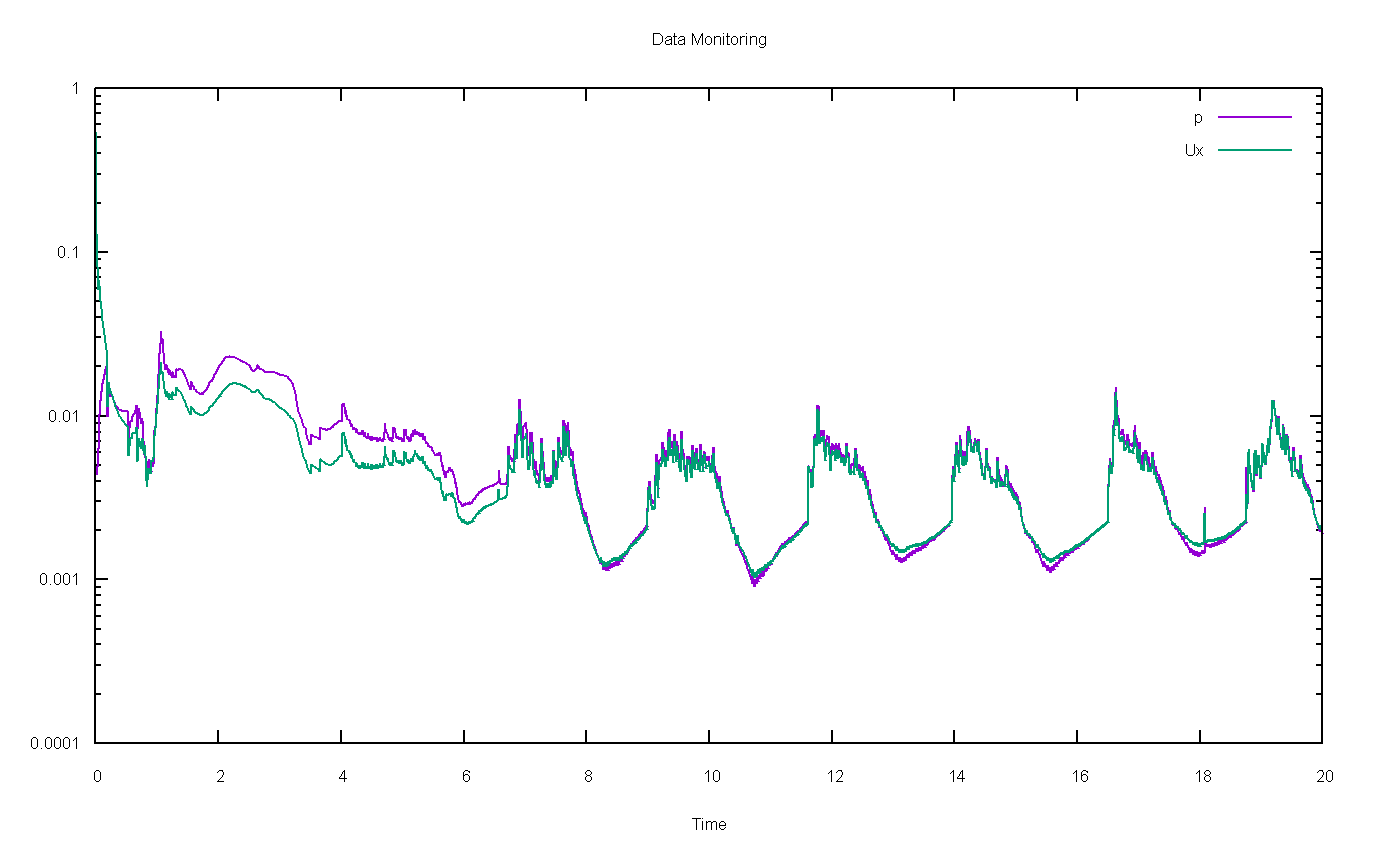
\includegraphics{41-residuals_foamMonitoring.png}
\caption[Ejemplo de visualización de residuos con \emph{foamMonitoring}]{Ejemplo de visualización de residuos con \emph{foamMonitoring}, para las variables \emph{p} y \emph{Ux}}
\label{fig:residuals_foamMonitoring}
\end{figure}

Otra forma para visualizar los residuos, es siguiendo los pasos de la
instalación del paquete
\href{http://openfoamwiki.net/index.php/Contrib/PyFoam}{PyFoam}. Esta
opción resulta mucho más sencilla, dado que no se requiere ninguna
configuración adicional en el caso, está preconfigurado para analizar
las variables principales implicadas en el caso. Basta con ejecutar el
código de resolución en segundo plano y introducir la orden:
\texttt{pyFoamPlotWatcher.py\ log.interFoam}

\begin{figure}
\centering
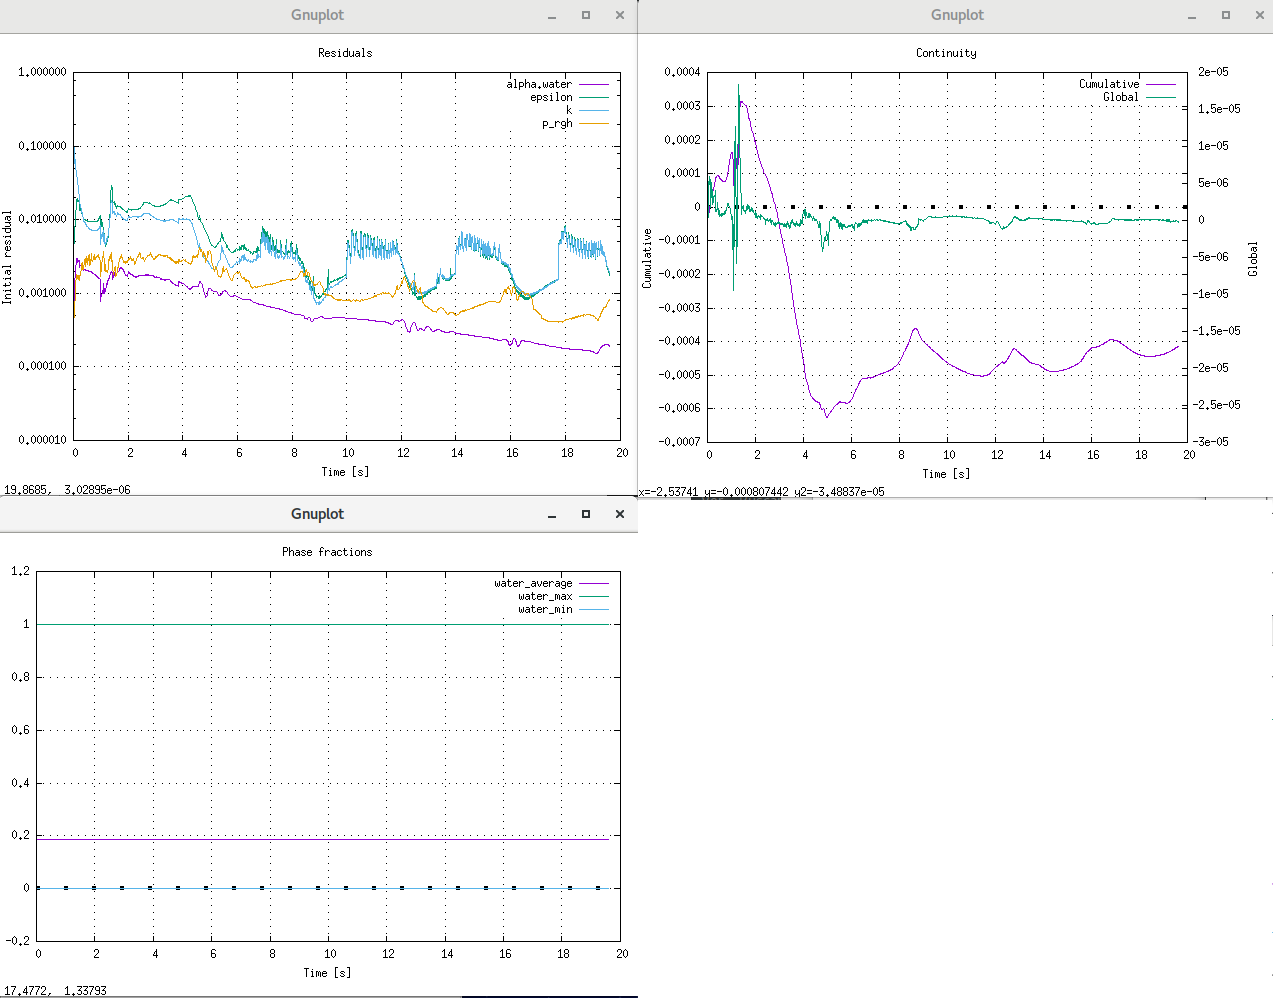
\includegraphics{41-residuals_py220.png}
\caption{Ejemplo de visualización de residuos con \emph{pyFoam}}
\label{fig:residuals_py220}
\end{figure}
